\section{Multistage architecture}
\label{sec:multistage}

\begin{figure}[!htpb]
  \begin{center}
    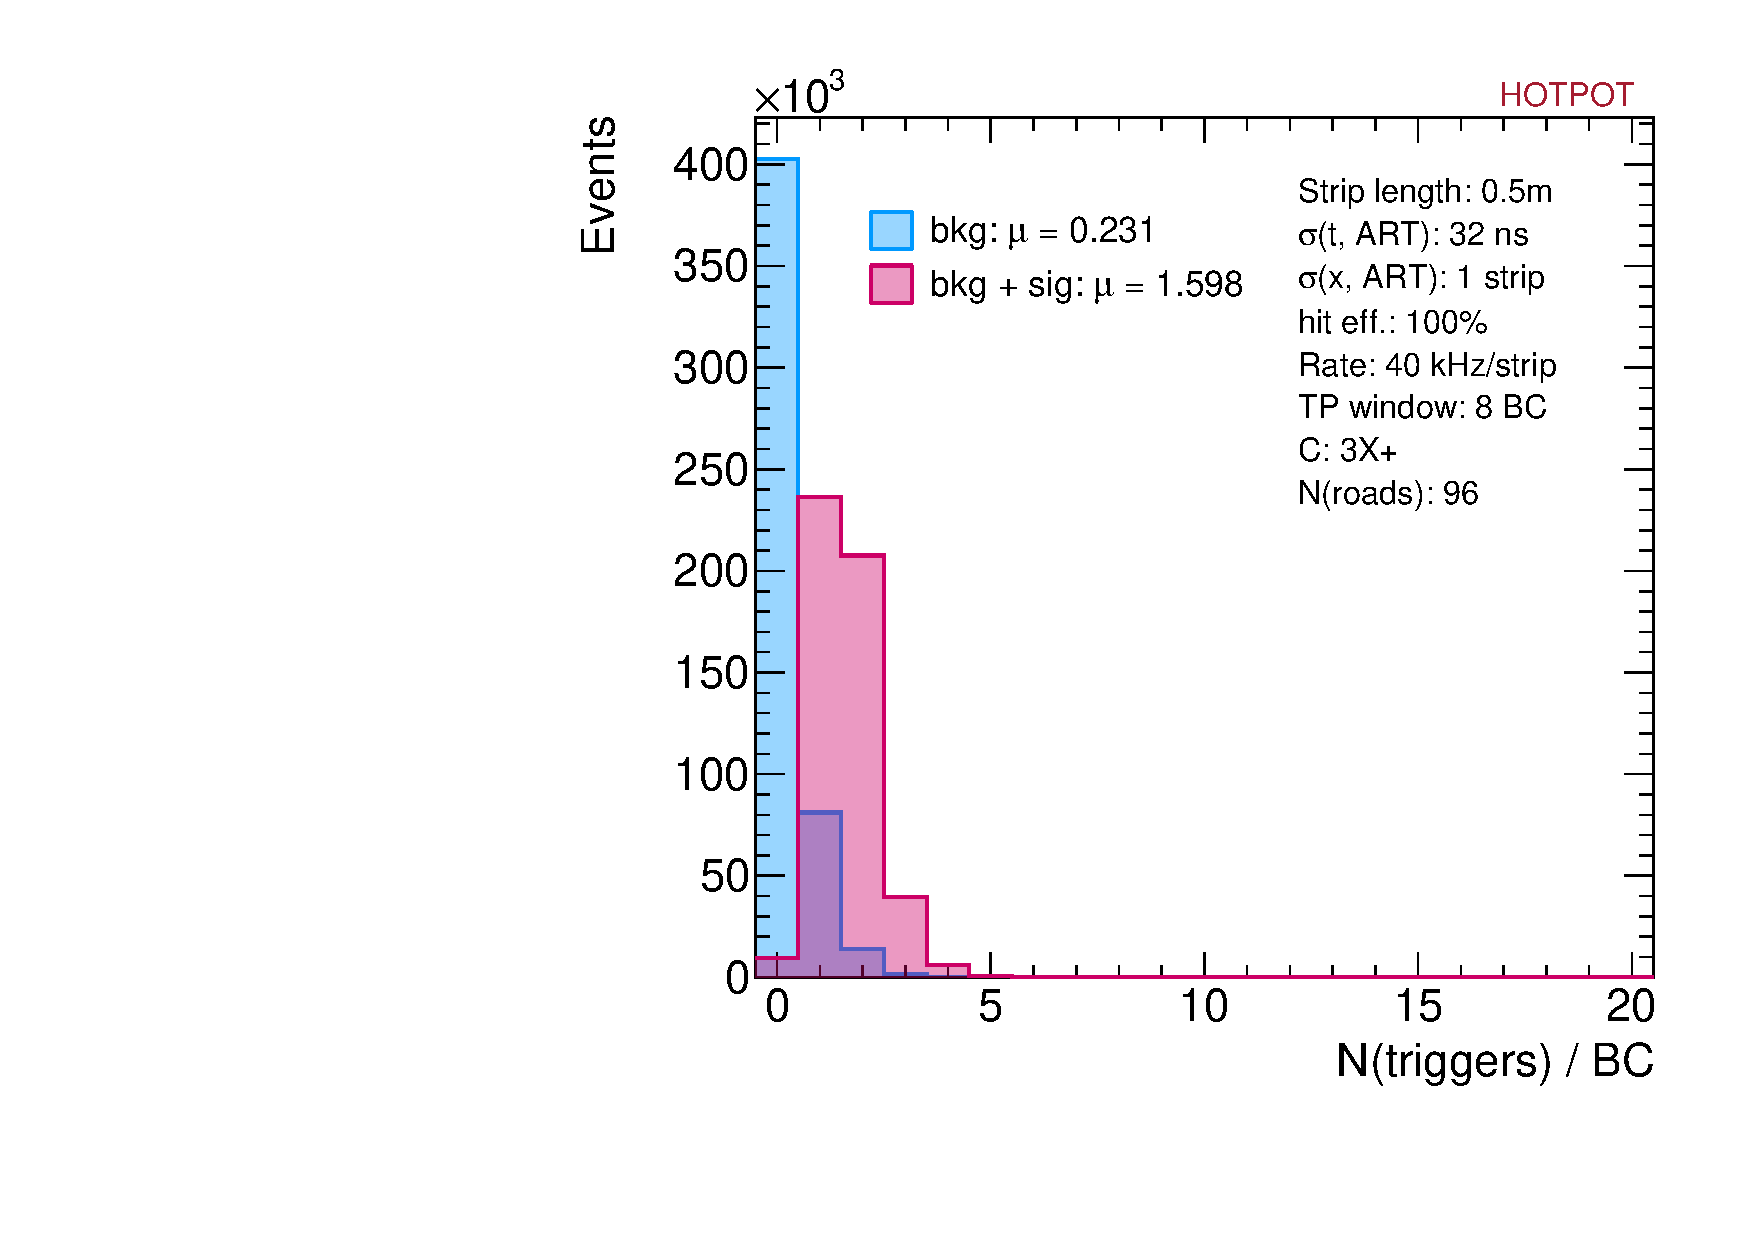
\includegraphics[width=0.48\textwidth]{figures/small_3x0uv_ntrig_BC7.pdf}
    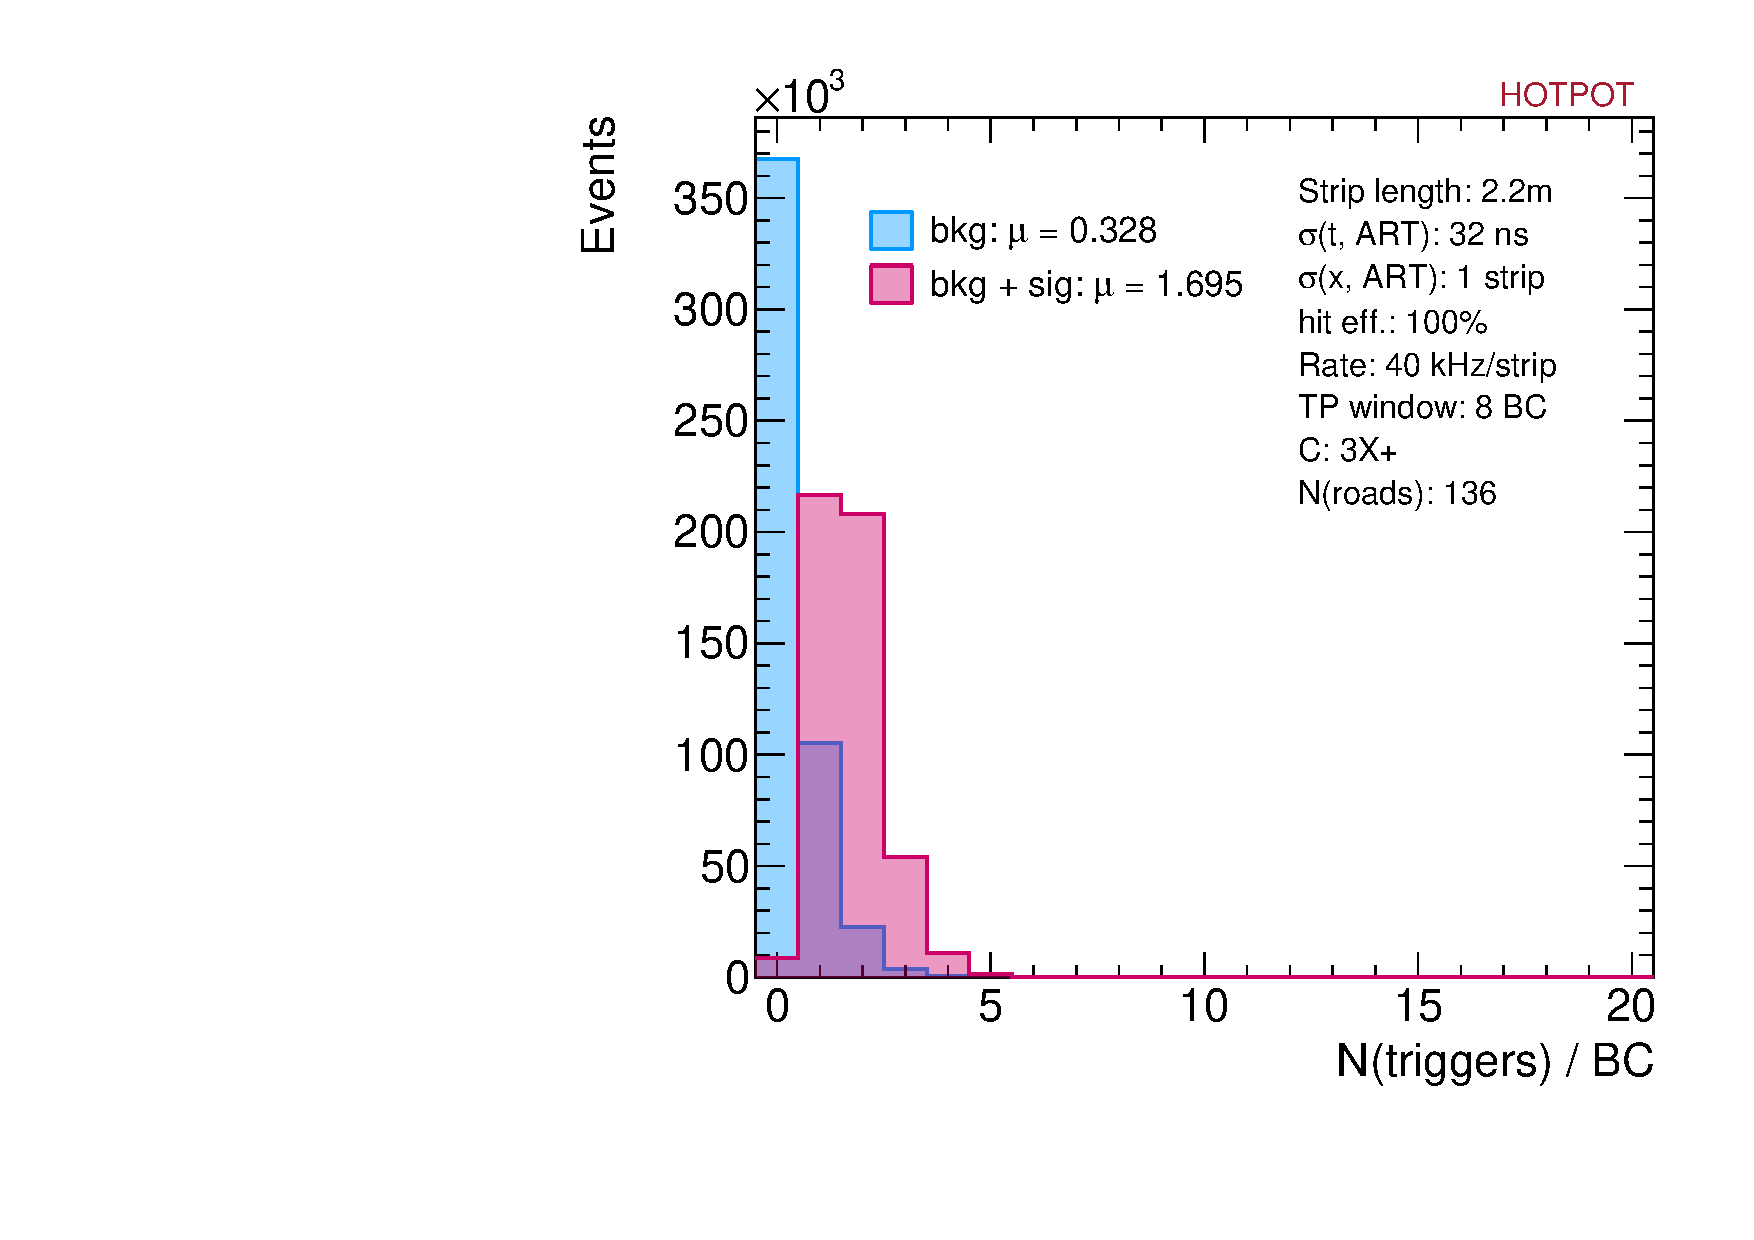
\includegraphics[width=0.48\textwidth]{figures/large_3x0uv_ntrig_BC7.pdf}
  \end{center}
  \vspace{-10pt}
  \caption{Number of triggers found per BC for 0.5m long strips (left) and 2.2m long strips (right) with a 3X requirement. The blue histogram represents the distribution if we only have uncorrelated background hits, and the pink histogram represents the distribution if we also add a muon track. For the pink histogram, since number of triggers in a given BC is dependent on the BC, we pick the BC when the first real muon ART hit is 8 BCs old.}
  \label{fig:3x_trig}
\end{figure}

With the proposed algorithm modifications using small stereo roads, a multistage trigger finder is currently implemented to reduce redundant processing. In order to avoid the scaling of having many unique pairs of $U$, $V$ roads per X road, a stage I filter for triggers is applied. In this stage, we look for 3X coincidences with no requirement on the ages of the ART hits. This narrows the set of X roads. Then, in stage II, we look for 3X3UV+ coincidences in $U$, $V$ roads associated to the pre-filtered set of X roads. We also require that one of the ART hits is ``mature", or 8 BCs old in the buffer which collects ART hits. The caveat of this multistage filtering setup is that the number of $X$ roads in the pre-filtered set must be limited to a set number, \textit{n}. A similar limit, \textit{m}, also applies to the number of 3X3UV coincidences that can be processed per corresponding X road. $n \times m$ must be fewer than 8, a number which is determined by the mother clock in the MMTP implementation. Figure \ref{fig:mstage} illustrates this scheme.

\begin{figure}[!htpb]
  \begin{center}
    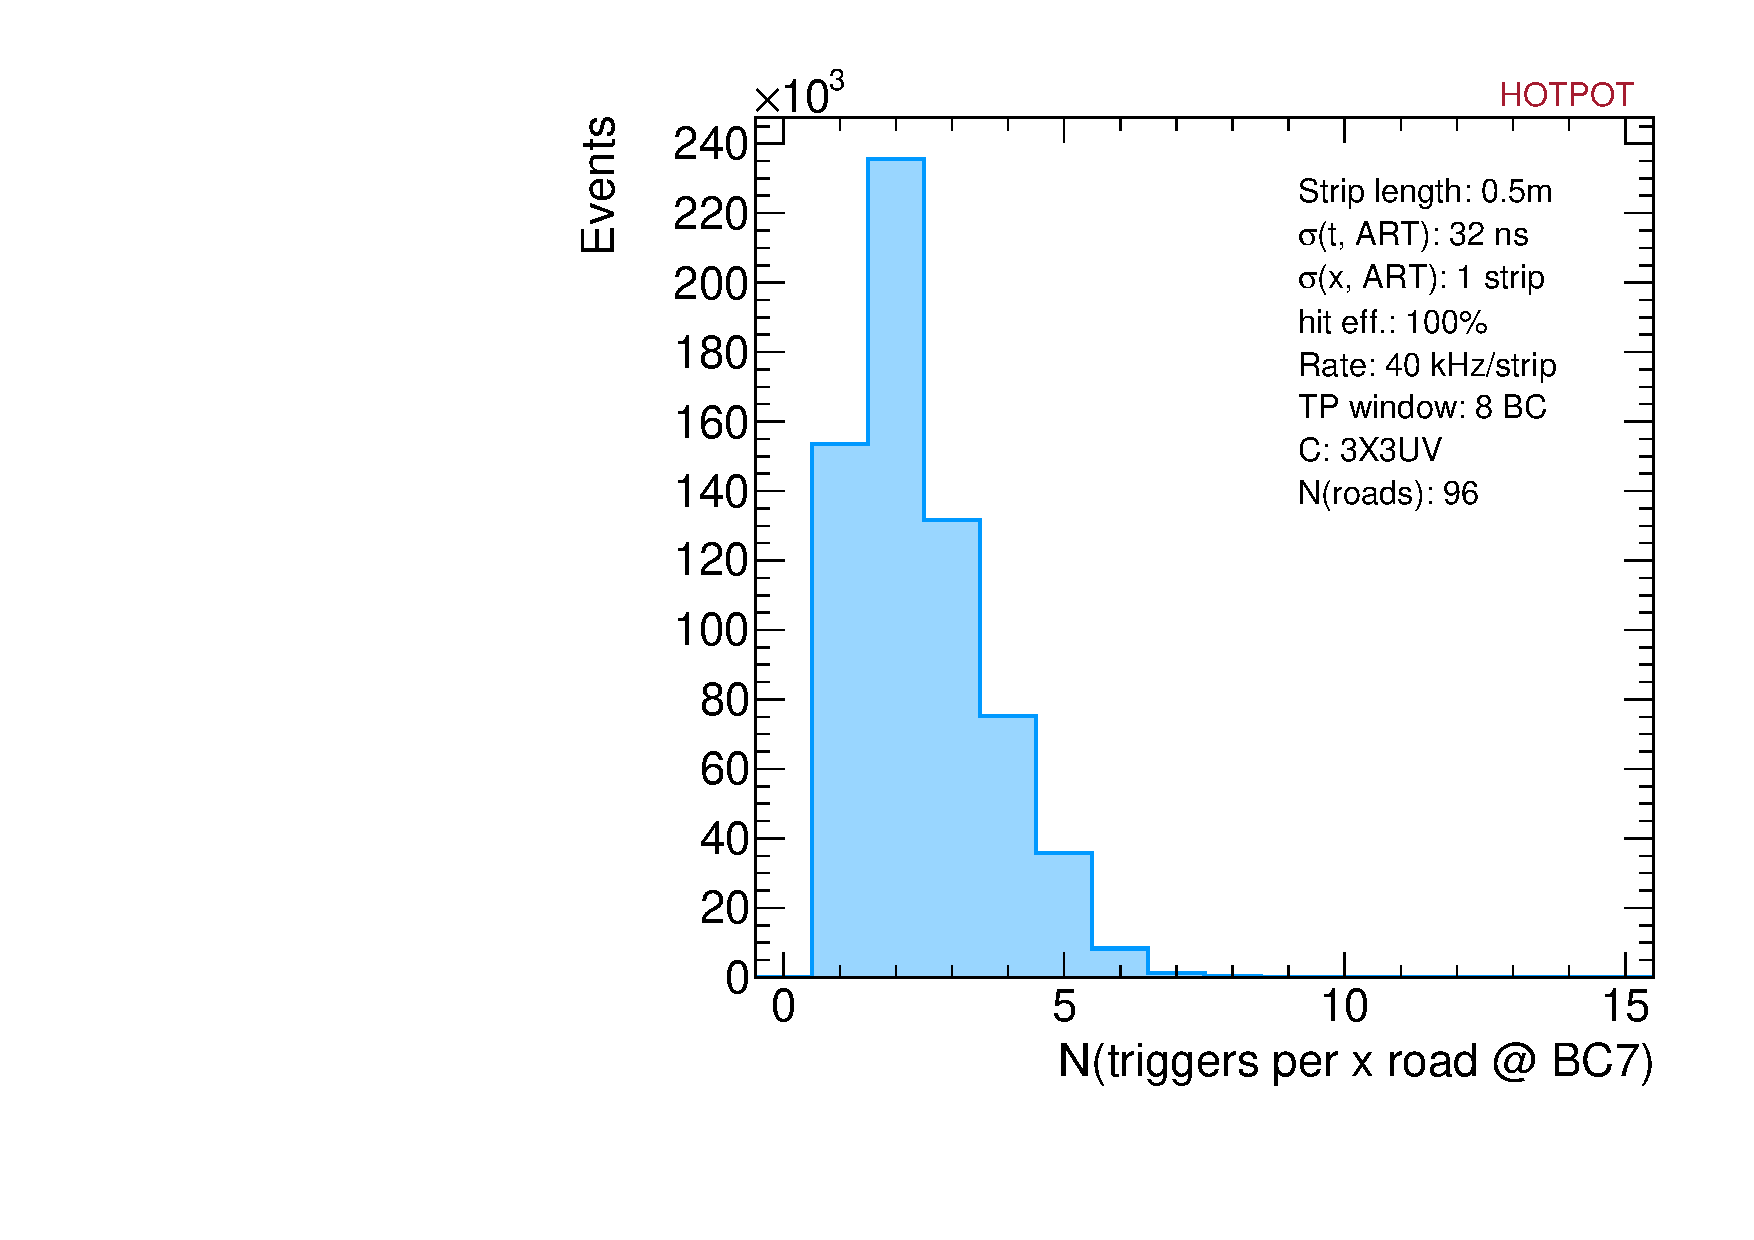
\includegraphics[width=0.48\textwidth]{figures/small_trigs_per_x.pdf}
    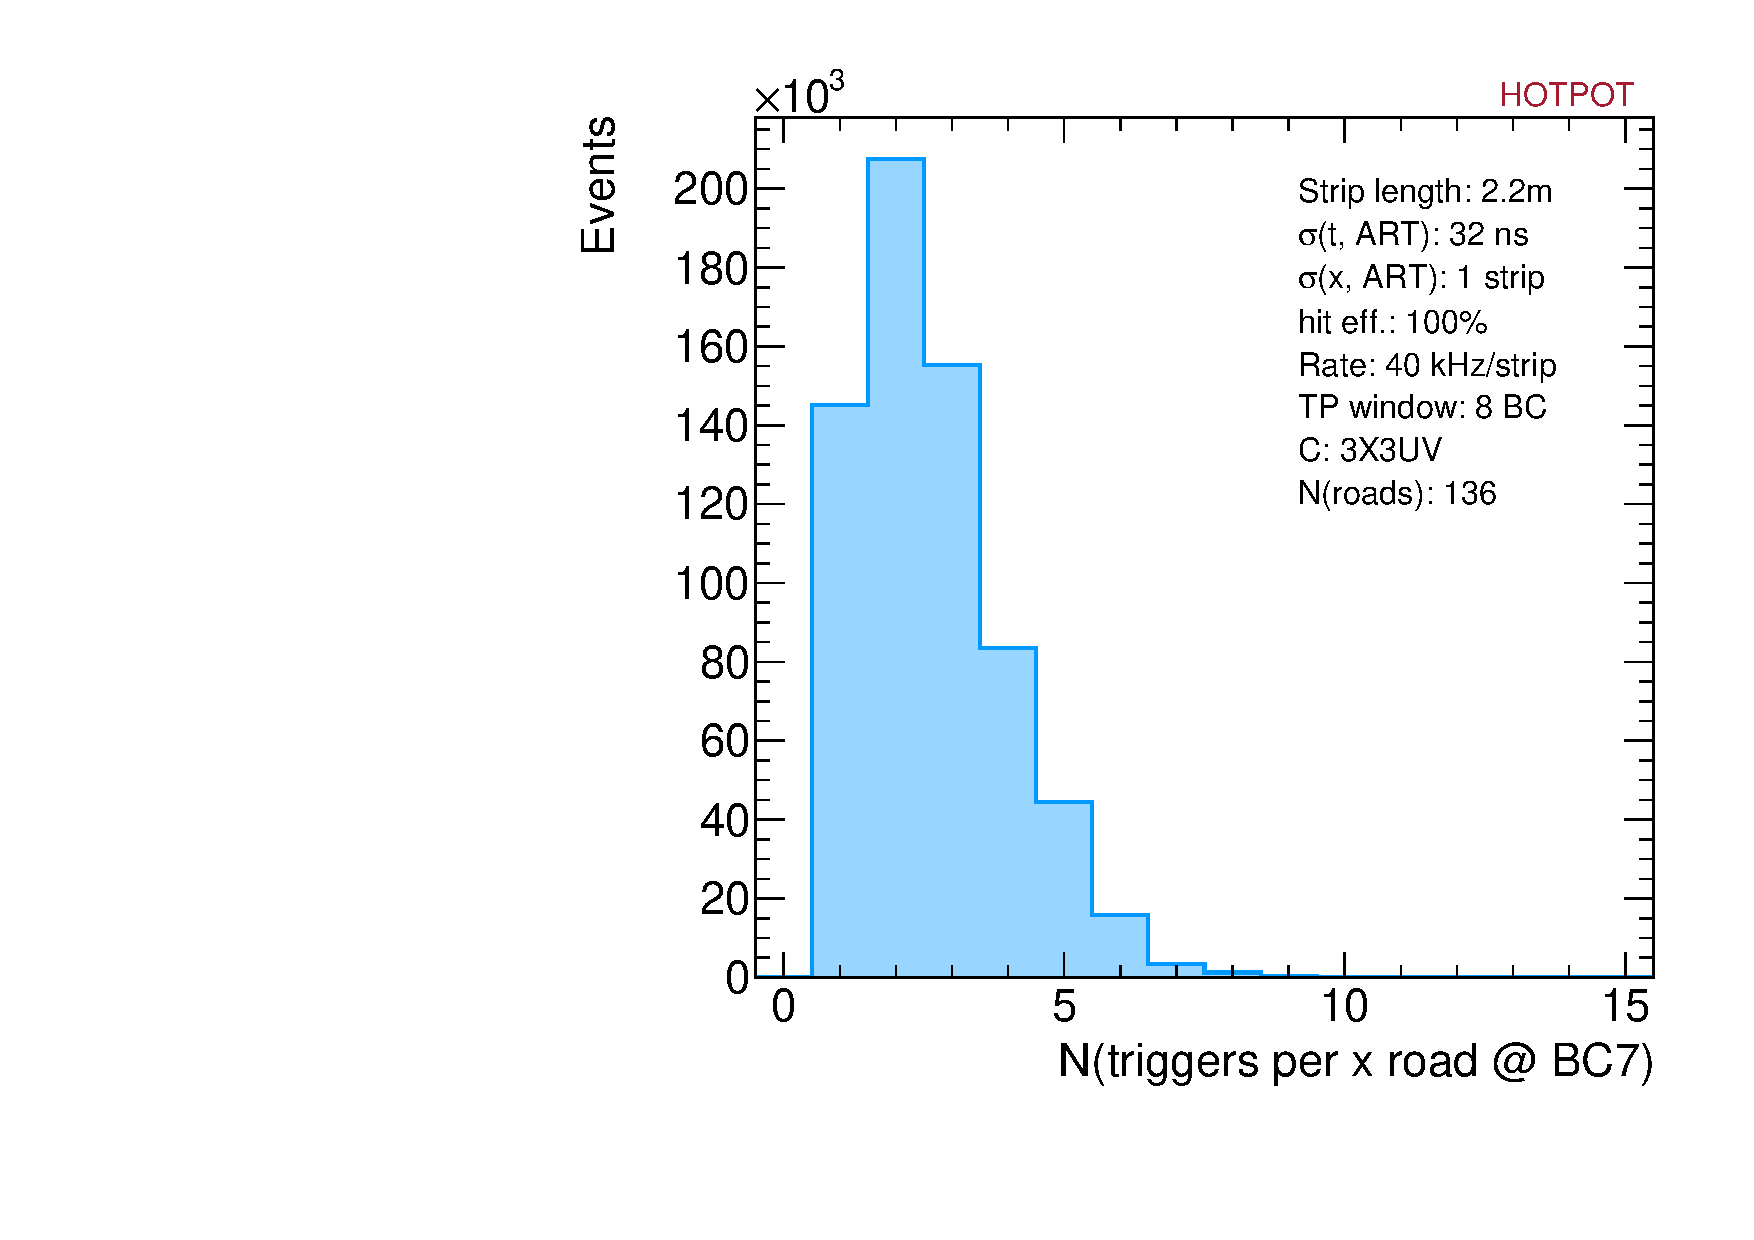
\includegraphics[width=0.48\textwidth]{figures/large_trigs_per_x.pdf}
  \end{center}
  \vspace{-10pt}
  \caption{Number of triggers found per BC associated to a given $X$ road for 0.5m long strips (left) and 2.2m long strips (right) with a 3X3UV requirement. }
  \label{fig:trig_per_x}
\end{figure}

\begin{figure}[!htpb]
  \begin{center}
    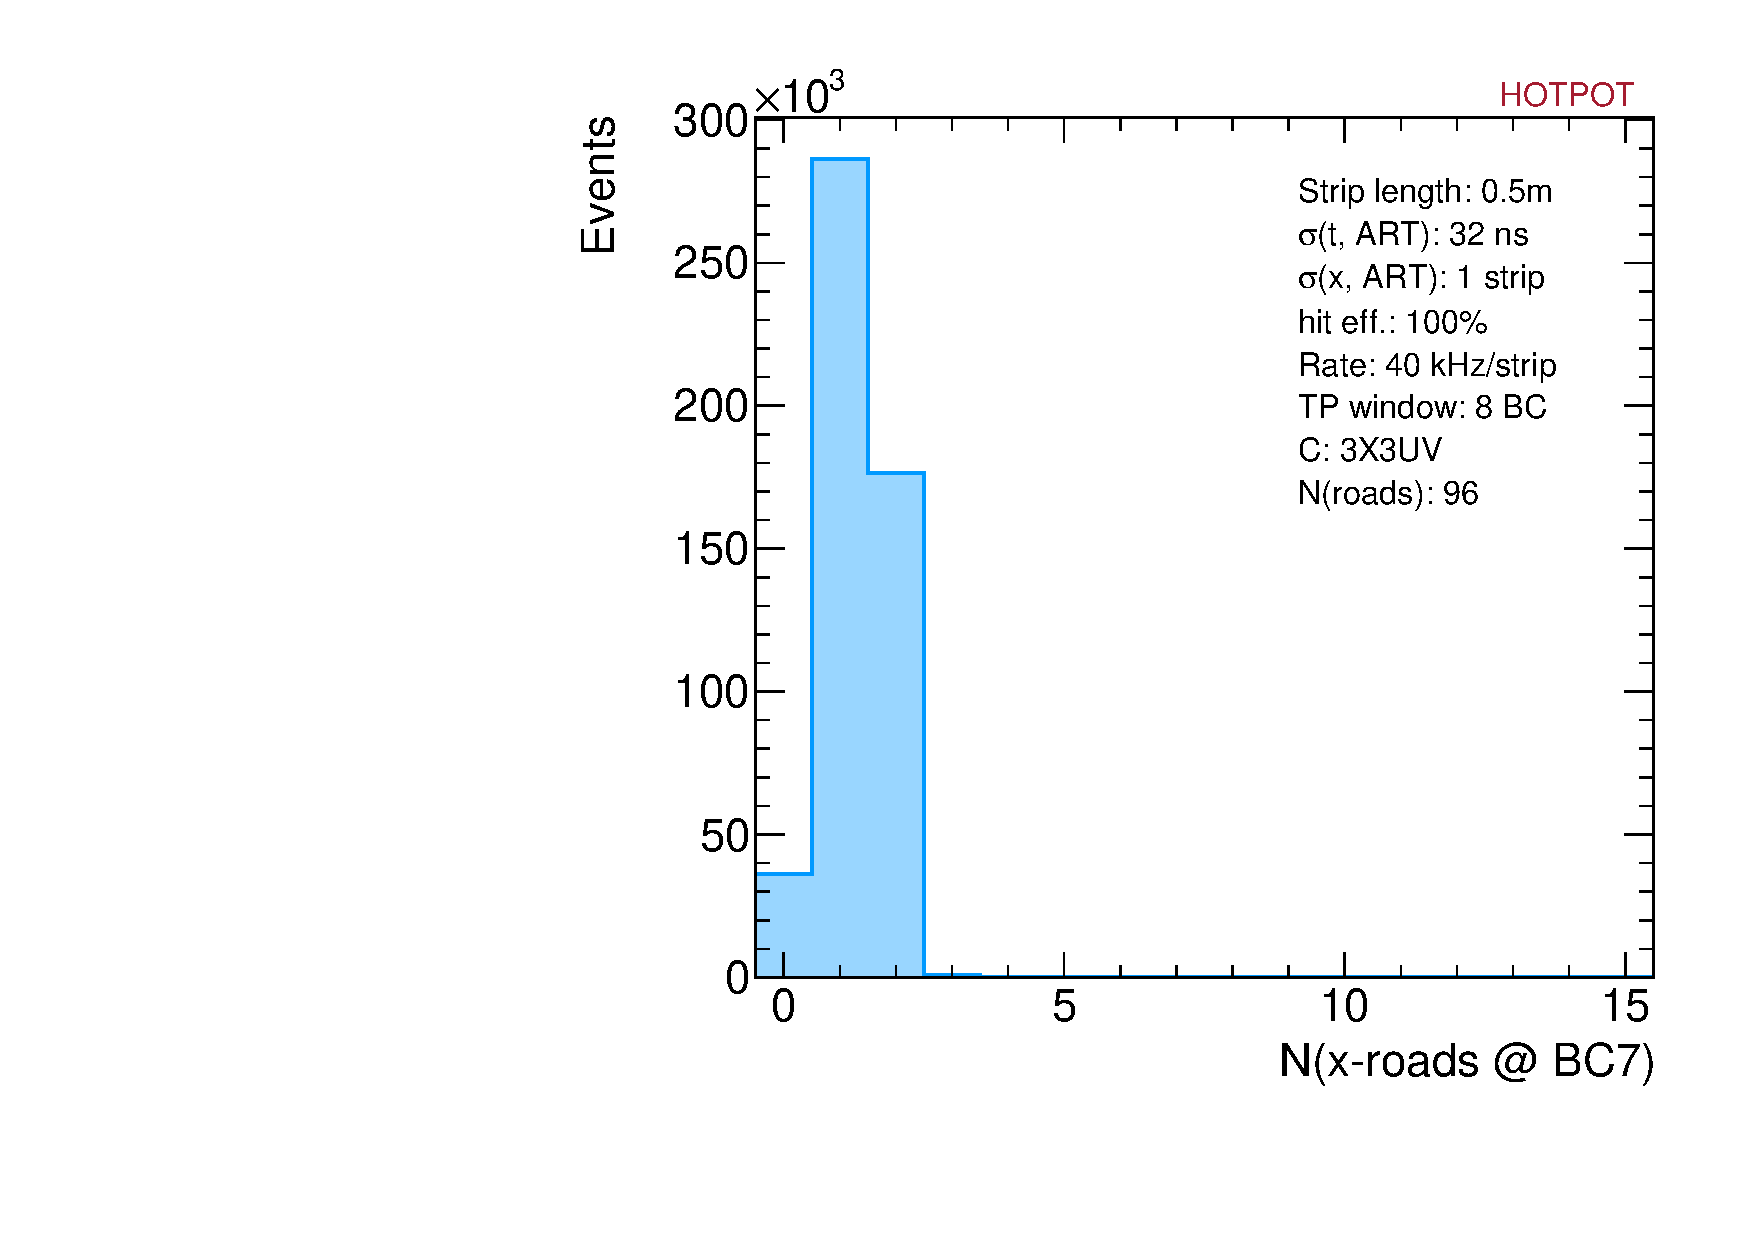
\includegraphics[width=0.48\textwidth]{figures/small_xroads.pdf}
    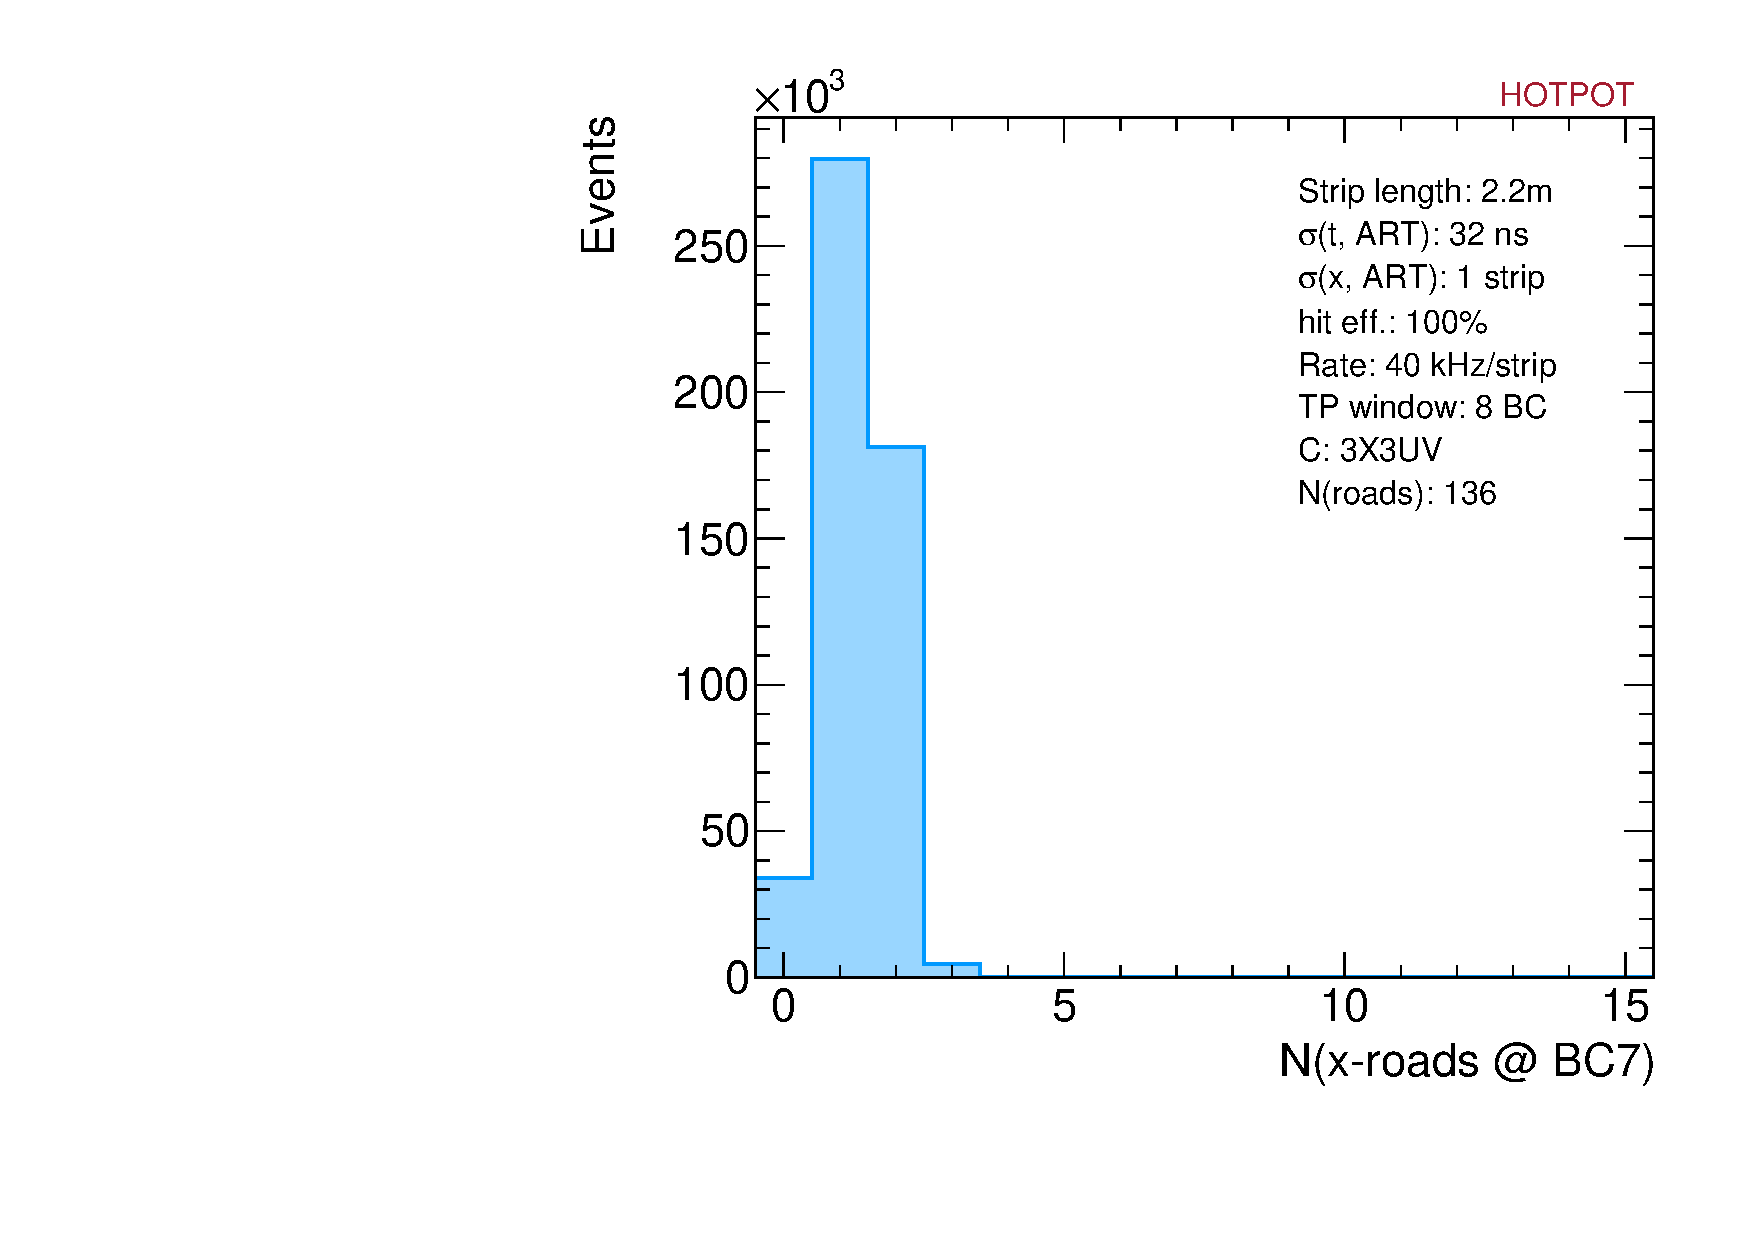
\includegraphics[width=0.48\textwidth]{figures/large_xroads.pdf}
  \end{center}
  \vspace{-10pt}
  \caption{Number of $X$ roads found per BC for 0.5m long strips (left) and 2.2m long strips (right) with a 3X3UV requirement. }
  \label{fig:xroads}
\end{figure}

Figure \ref{fig:3x_trig} shows the number of expected triggers found at the 3X stage if we assume 40 kHz of uncorrelated background. Again, we look at the BC in which the first real muon hit has been in the MMTP buffer for 8 BCs. The distribution, when there is a real muon track, has a tail up to 5 $X$ roads triggering in a given BC. Figure \ref{fig:trig_per_x} shows the distribution of 3X3UV triggers associated to a single $X$ road, which can be as many as 9-10. However, if we look at the number of unique $X$ roads associated to the 3X3UV triggers, shown in Fig. \ref{fig:xroads}, we see that the distribution peaks at a smaller value than the number of 3X triggers, shown in Fig. \ref{fig:3x_trig}. This indicates that a significant portion of the $X$ roads which pass the stage I pre-filter do not form stage II triggers.
\begin{figure}[!htpb]
  \begin{center}
    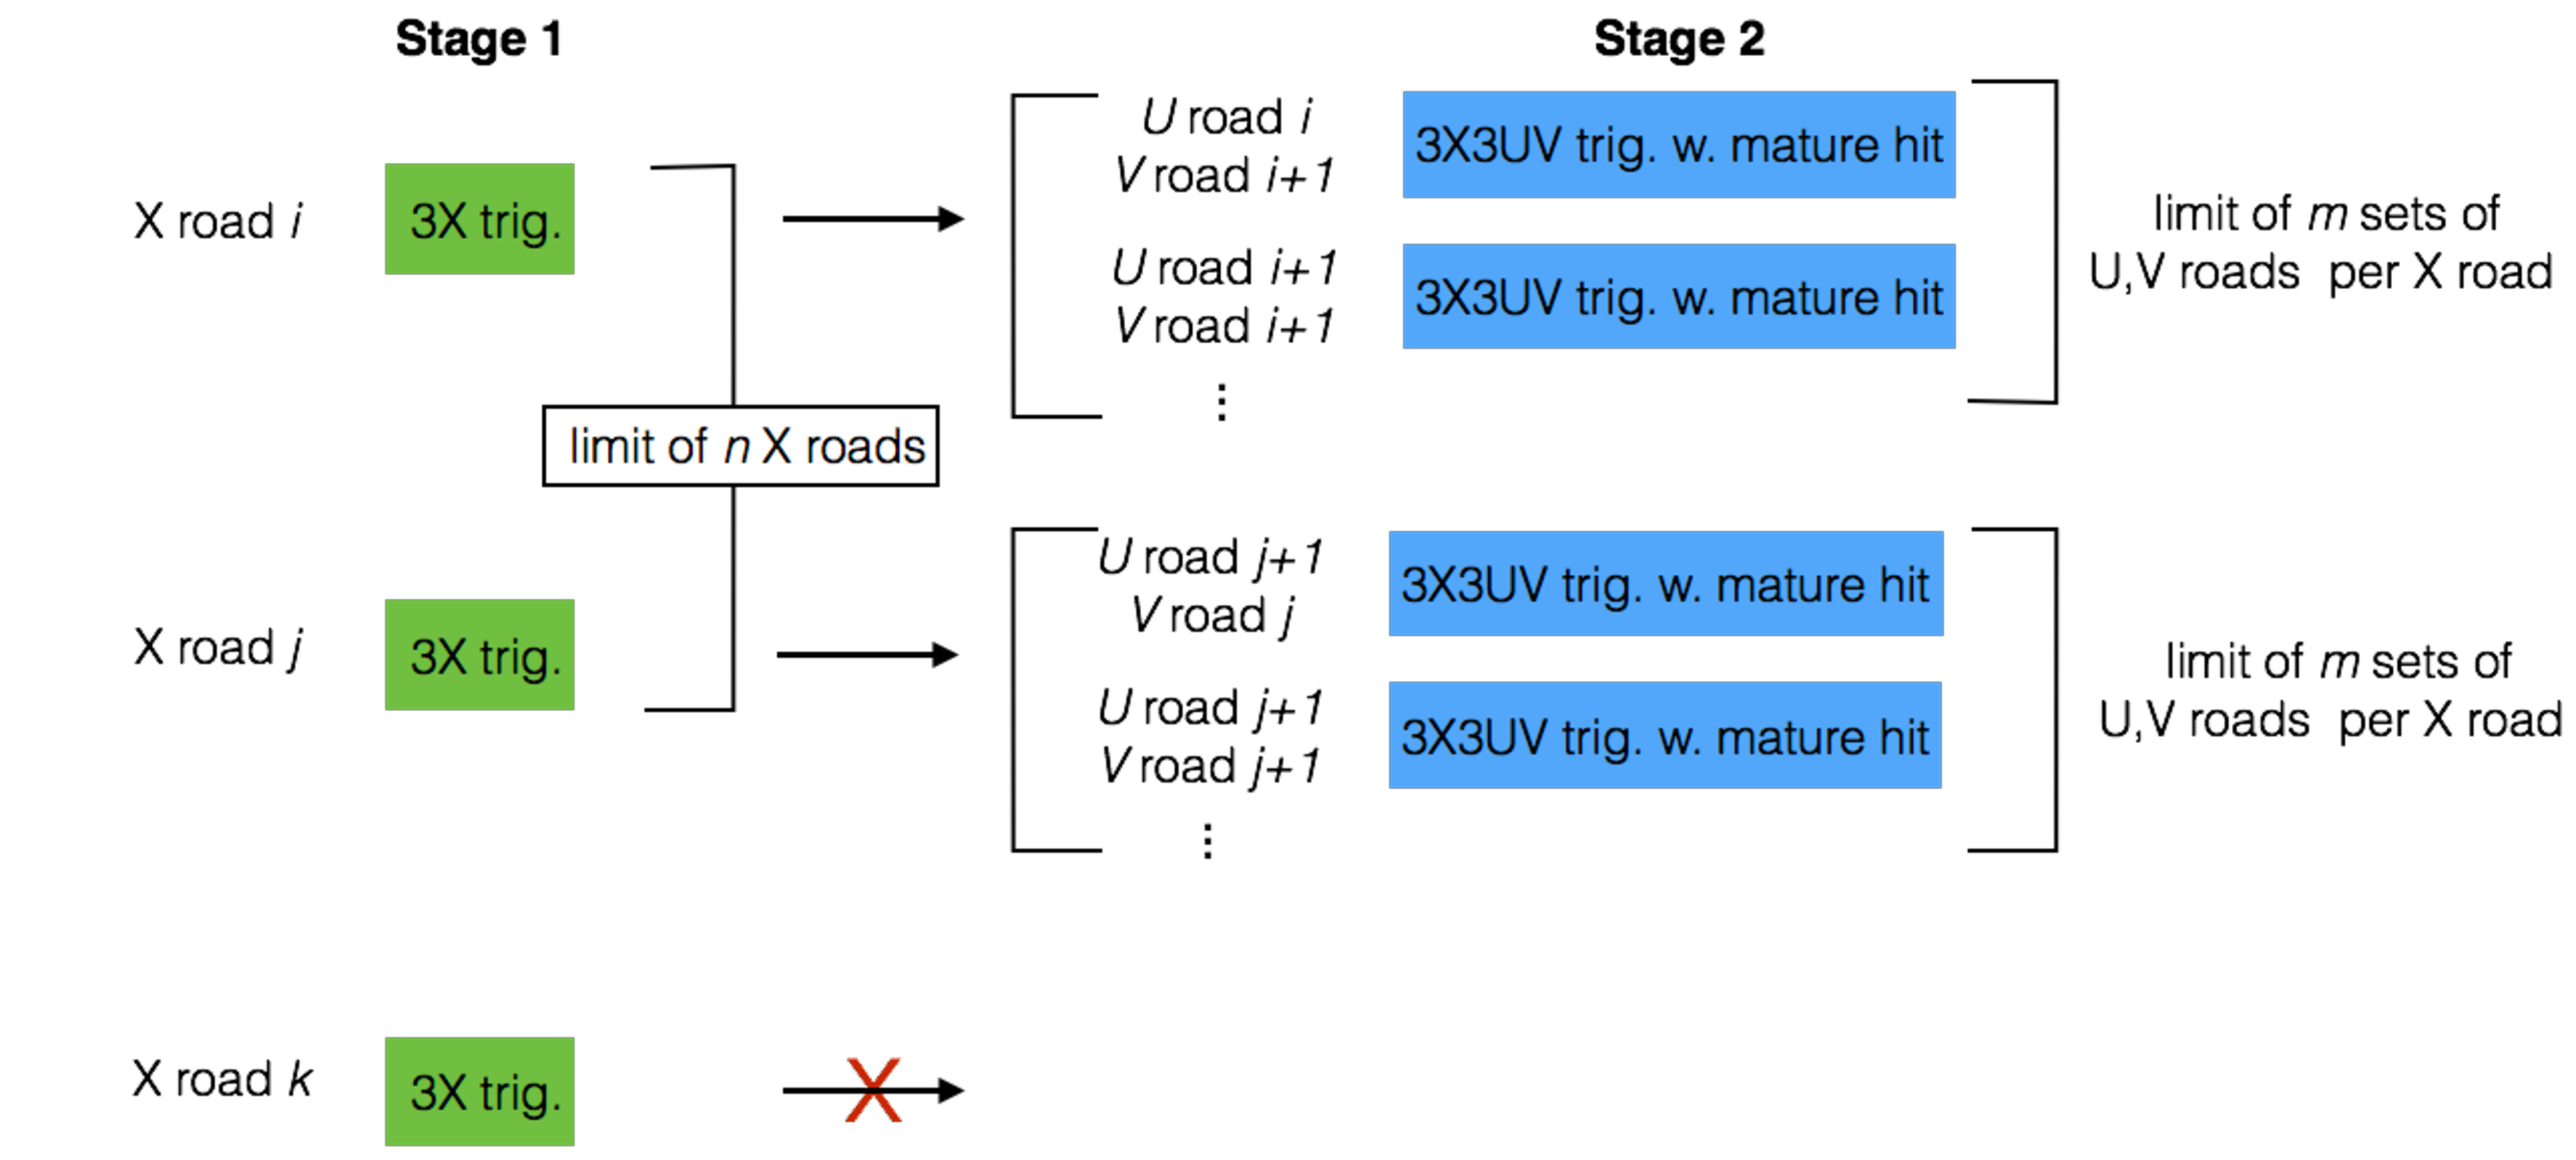
\includegraphics[width=0.96\textwidth]{figures/multistage.pdf}
  \end{center}
  \vspace{-10pt}
  \caption{Schematic of the two-stage filter for triggers. In stage I, up to \textit{n} X-roads with 3 x-plane hits are processed. In stage II, for each of these X-roads, the MMTP processes up to \textit{m} sets of $U$,$V$ roads. The total number $n \times m$ is currently limited to 8, set by the speed of the mother clock in the algorithm. }
  \label{fig:mstage}
\end{figure}
